\chapter{Sensitivity analysis other policies}
\label{app:2}
In this Appendix, the sensitivity analysis of the parameters discussed in Section \ref{analysis} will be presented for the remaining policies: battery subsidies, net billing and the annual offtake capacity tariff. 
\section{Residual load}
\subsection{Battery subsidies}
The data for the residual load sensitivity analysis of the battery subsidy policy (combined with the net metering policy) can be found in Figures \ref{fig:M}, \ref{fig:N}, \ref{fig:O} and \ref{fig:P}. 
\newline 
\begin{figure}[h!]
    \centering
    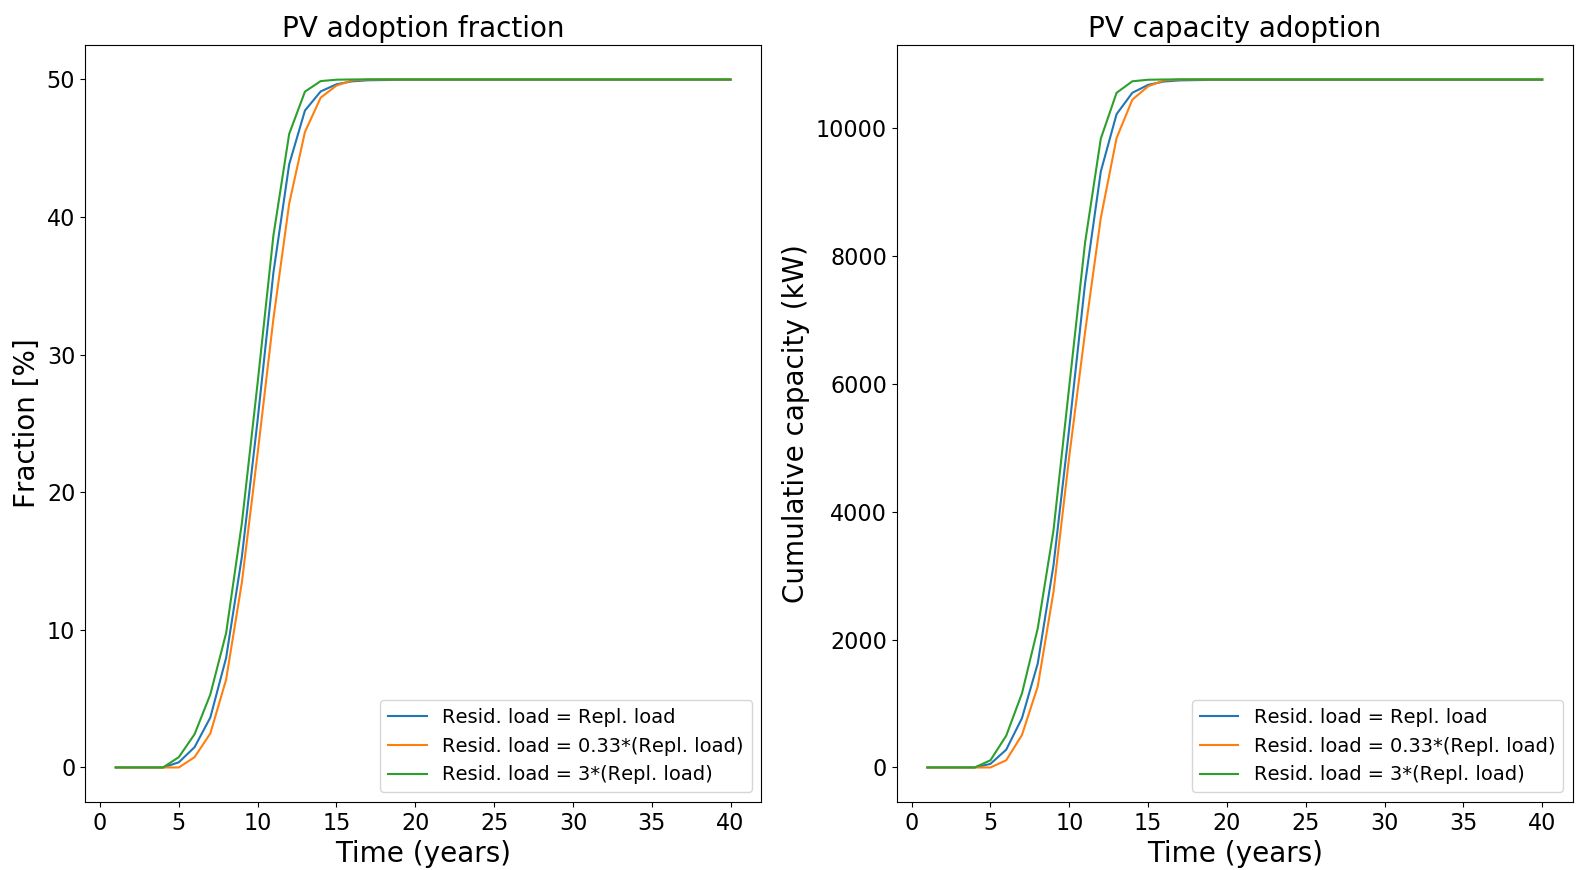
\includegraphics[width=10cm]{AppendixA/PVSubsresid.PNG}
    \caption{PV adoption for different residual loads}
    \label{fig:M}
\end{figure}
\noindent
\newline 
\begin{figure}[h!]
    \centering
    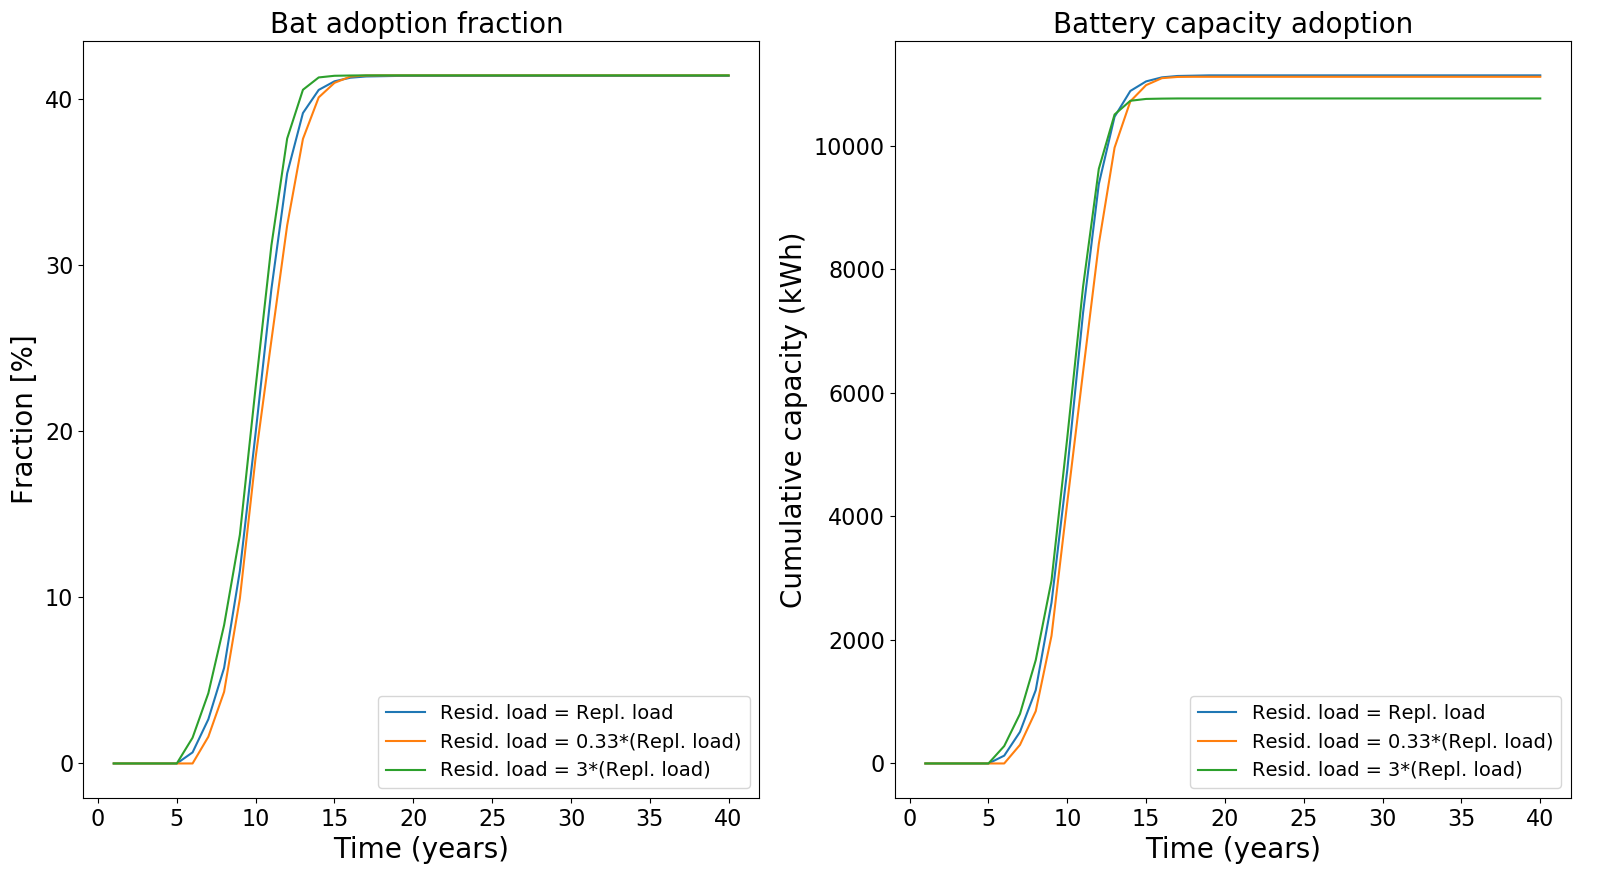
\includegraphics[width=10cm]{AppendixA/BatSubsresid.PNG}
    \caption{Battery adoption for different residual loads}
    \label{fig:N}
\end{figure}
\noindent
\newline 
\begin{figure}[h!]
    \centering
    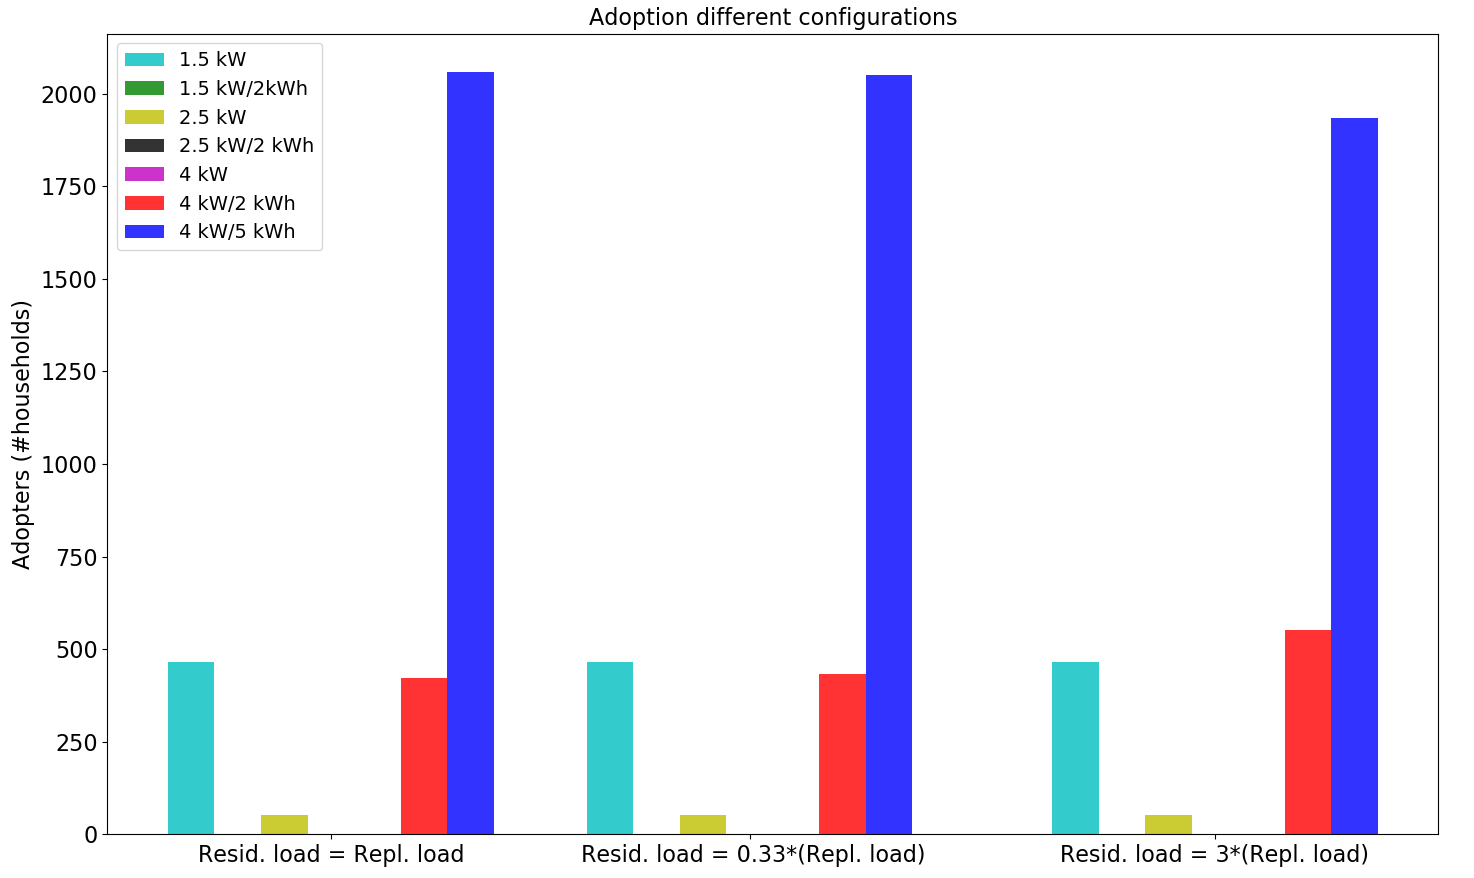
\includegraphics[width=10cm]{AppendixA/ConfigSubsresid.PNG}
    \caption{Configurations for different residual loads}
    \label{fig:O}
\end{figure}
\noindent
\newline
\begin{figure}[h!]
    \centering
    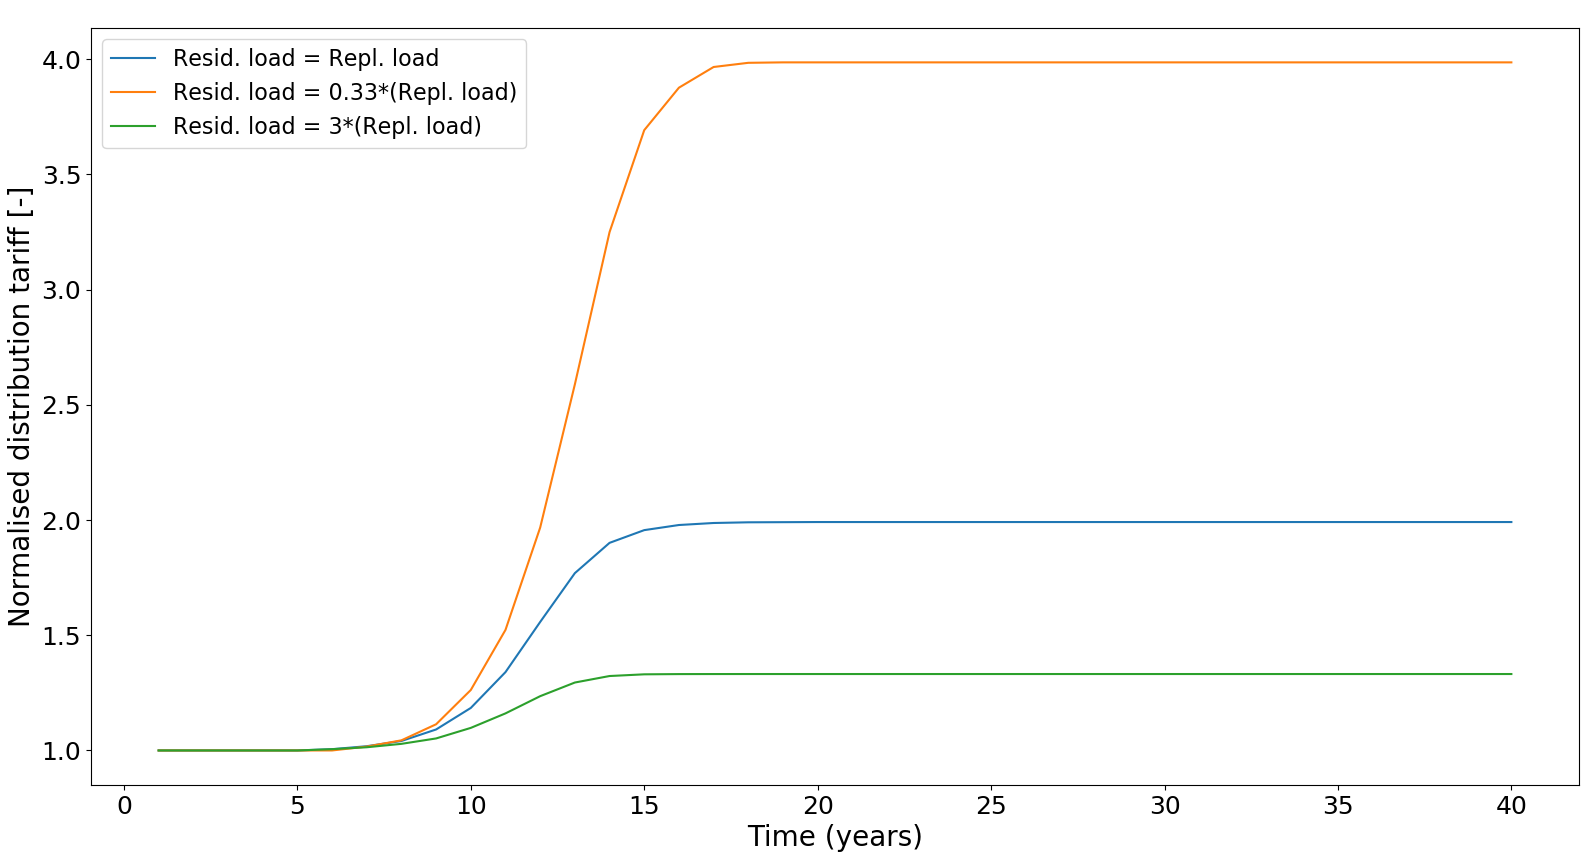
\includegraphics[width=10cm]{AppendixA/DistSubsresid.PNG}
    \caption{Normalised capacity tariff for different residual loads}
    \label{fig:P}
\end{figure}
\subsection{Net billing}
The data for the residual load sensitivity analysis of the net billing policy can be found in Figures \ref{fig:R}, \ref{fig:S}, \ref{fig:T} and \ref{fig:U}. 
\newline 
\begin{figure}[h!]
    \centering
    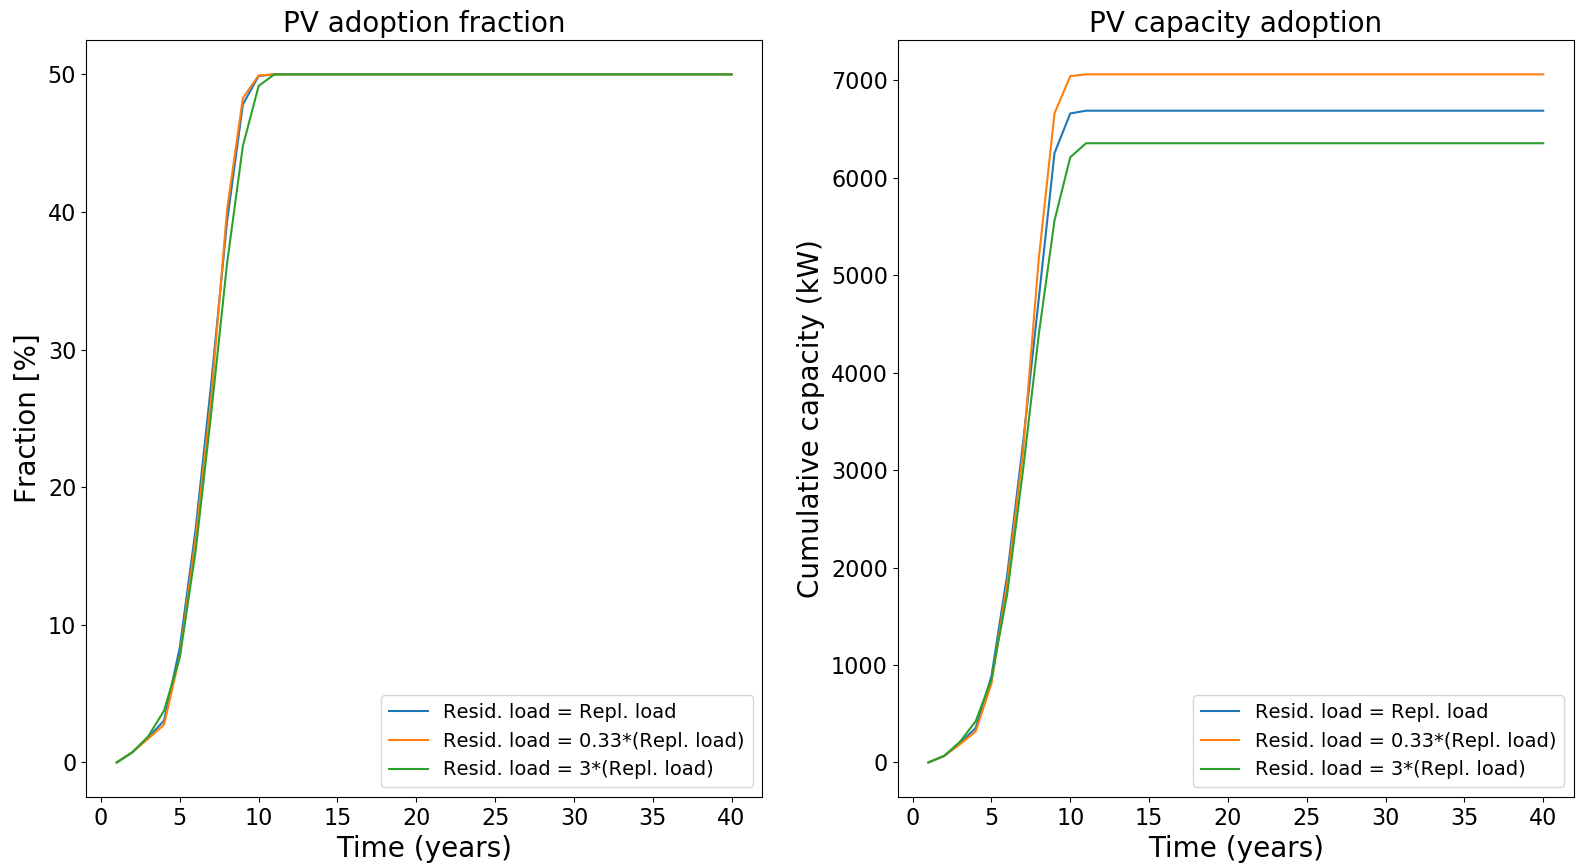
\includegraphics[width=10cm]{AppendixA/PVNBresid.PNG}
    \caption{PV adoption for different residual loads}
    \label{fig:Q}
\end{figure}
\noindent
\newline 
\begin{figure}[h!]
    \centering
    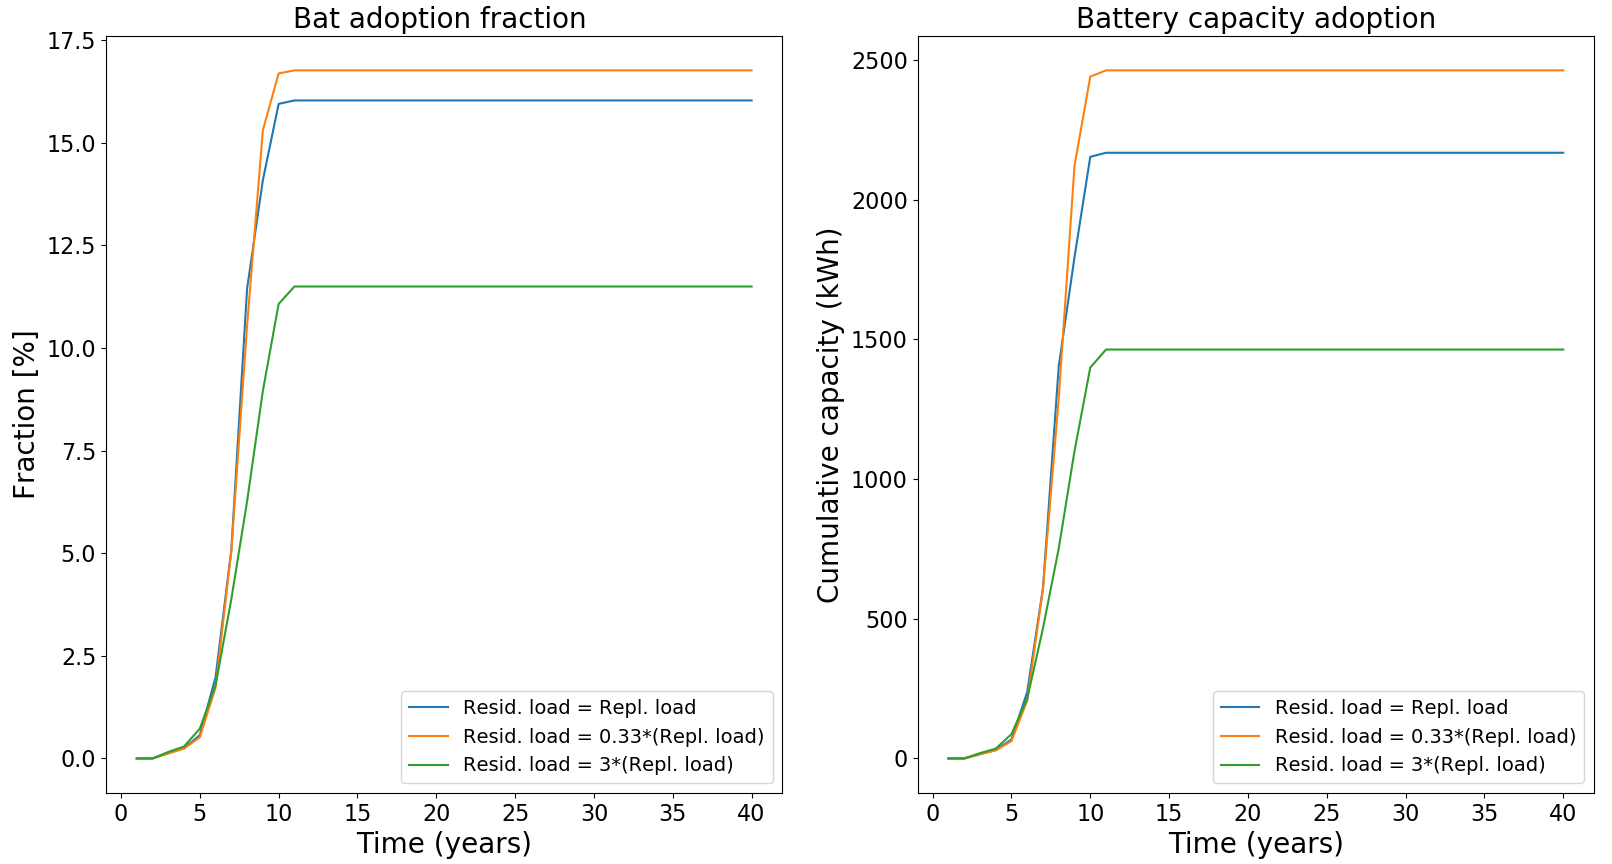
\includegraphics[width=10cm]{AppendixA/BatNBresid.PNG}
    \caption{Battery adoption for different residual loads}
    \label{fig:R}
\end{figure}
\noindent
\newline 
\begin{figure}[h!]
    \centering
    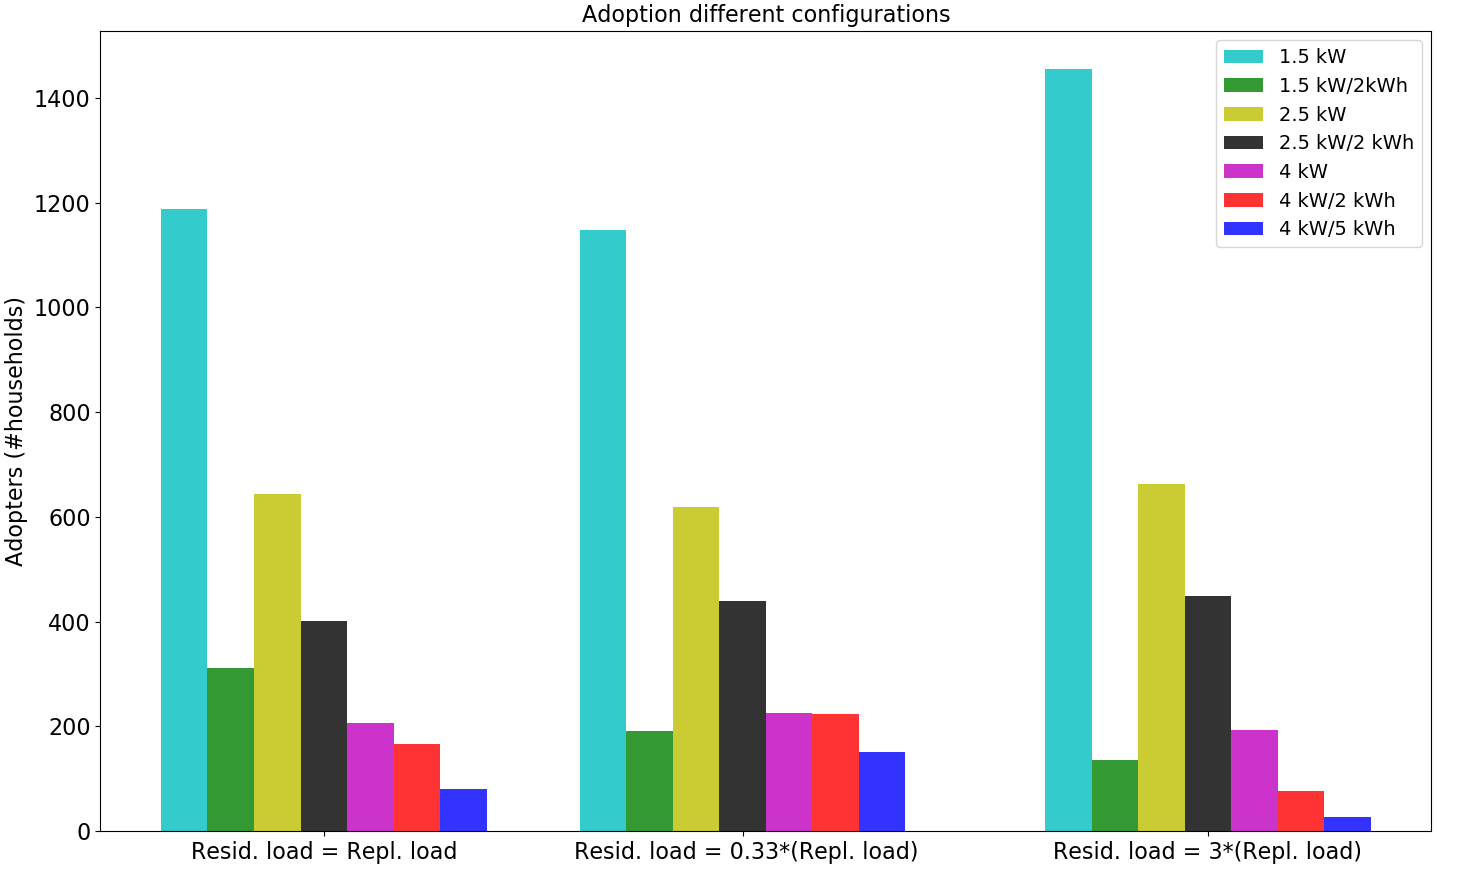
\includegraphics[width=10cm]{AppendixA/ConfigNBresid.PNG}
    \caption{Configurations for different residual loads}
    \label{fig:S}
\end{figure}
\noindent
\newline
\begin{figure}[h!]
    \centering
    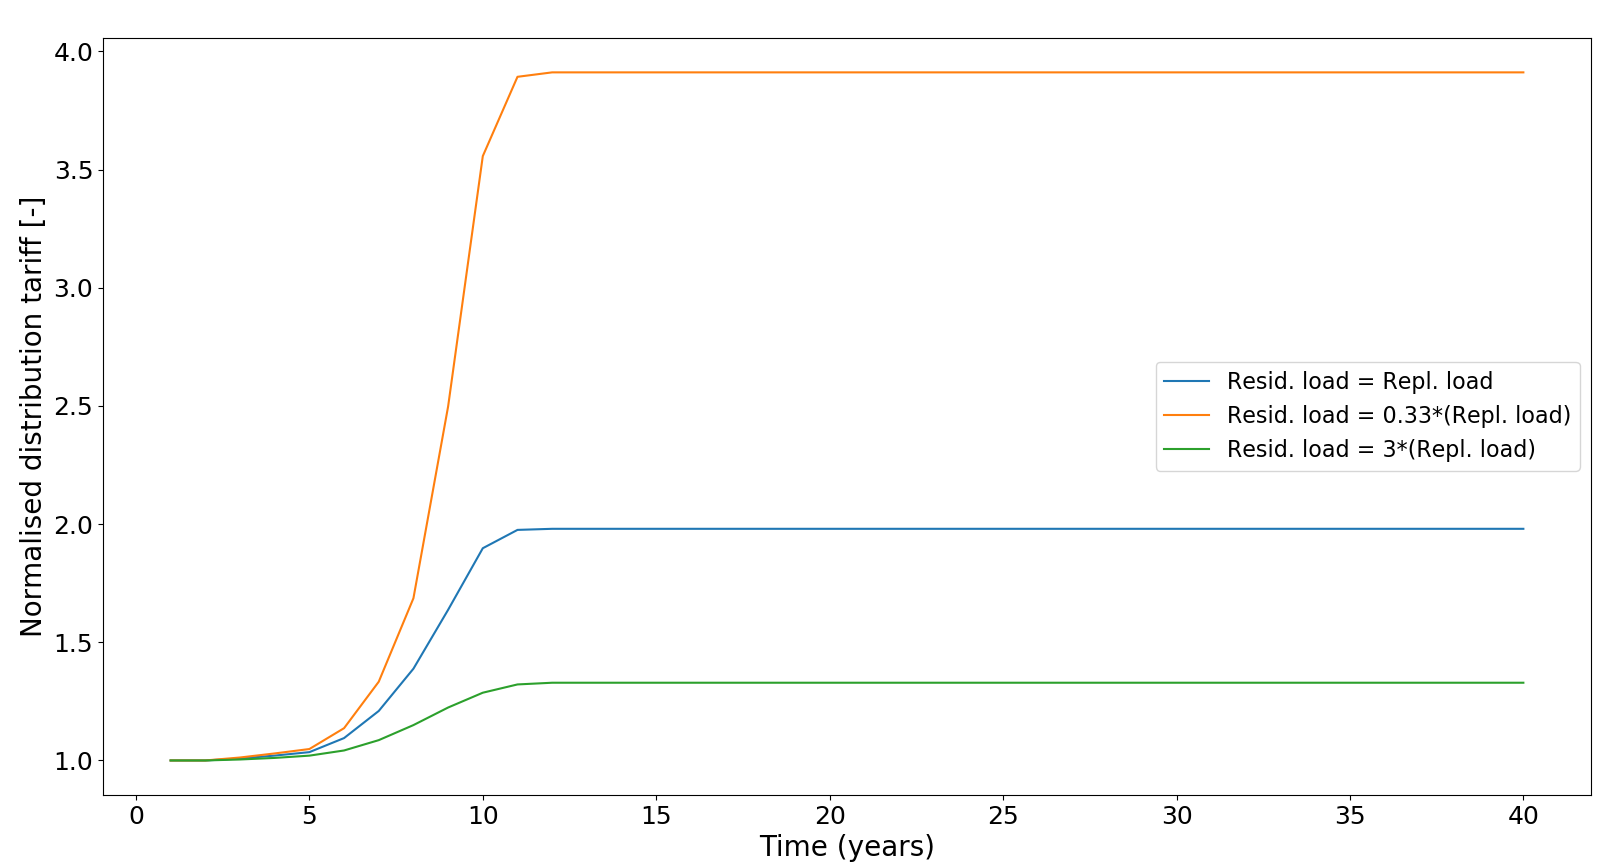
\includegraphics[width=10cm]{AppendixA/DistNBresid.PNG}
    \caption{Normalised capacity tariff for different residual loads}
    \label{fig:T}
\end{figure}%
\subsection{Annual capacity offtake}
The data for the residual load sensitivity analysis of the annual capacity offtake 
\newline 
\begin{figure}[h!]
    \centering
    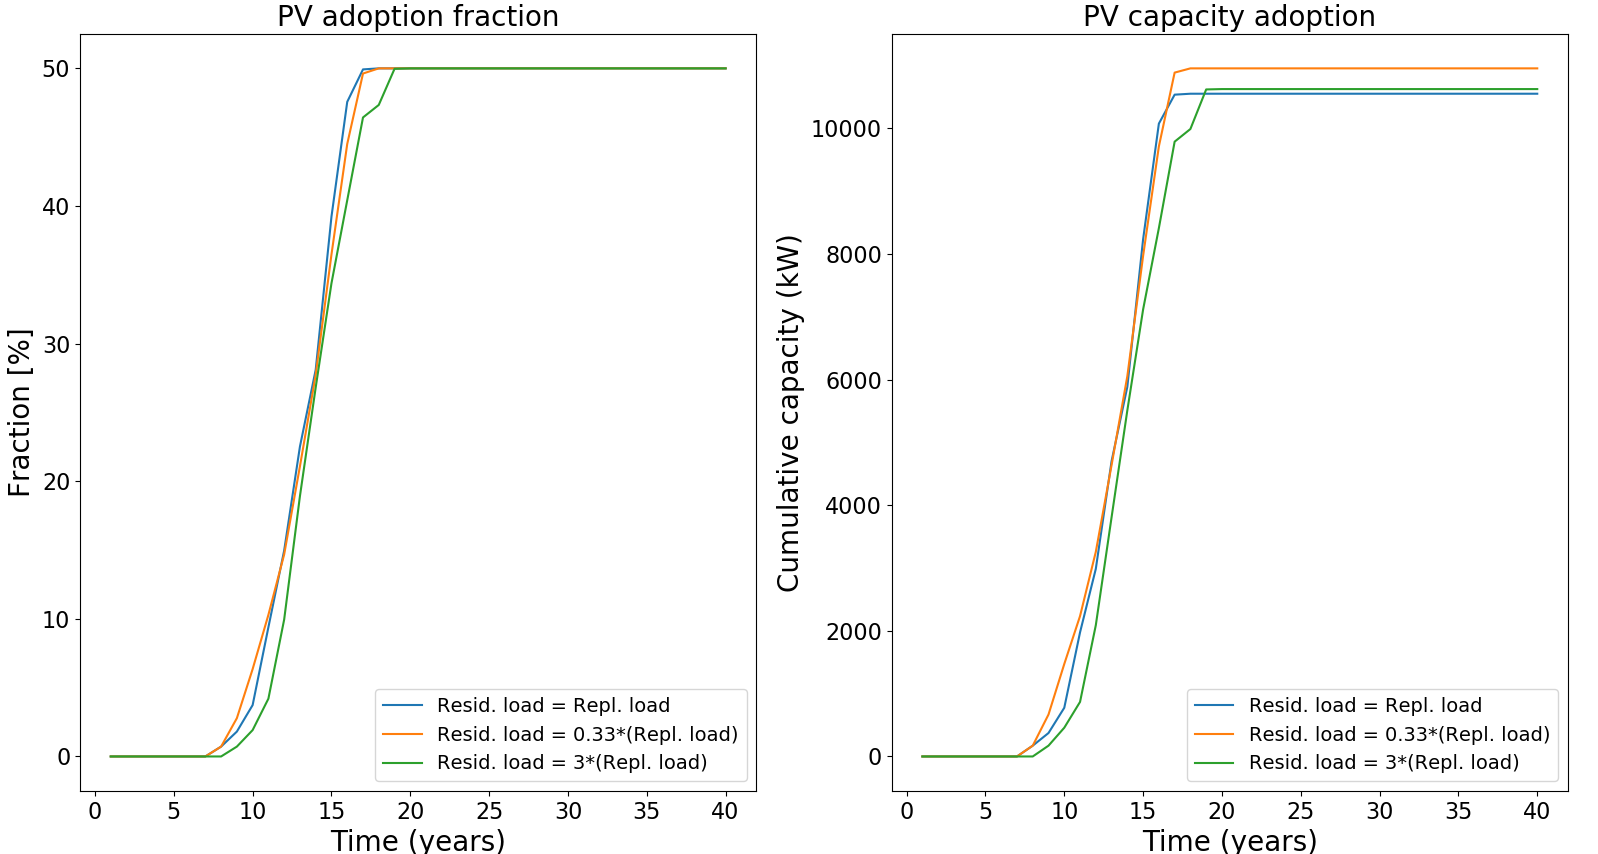
\includegraphics[width=10cm]{AppendixA/PVCapresid.PNG}
    \caption{PV adoption for different residual loads}
    \label{fig:U}
\end{figure}
\noindent
\newline 
\begin{figure}[h!]
    \centering
    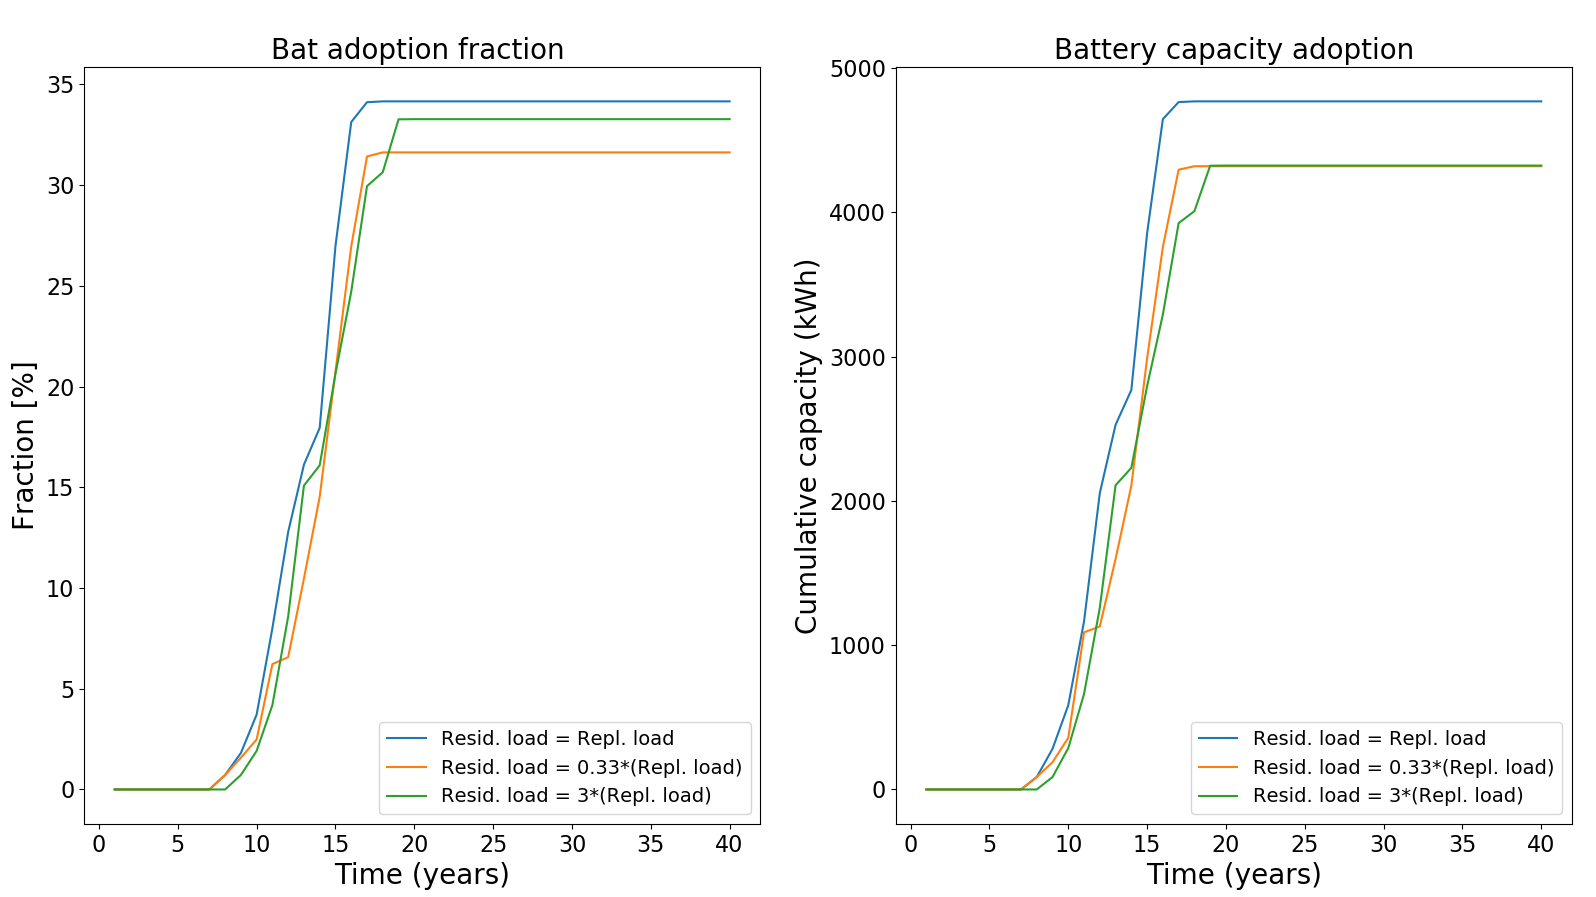
\includegraphics[width=10cm]{AppendixA/BatCapresid.PNG}
    \caption{Battery adoption for different residual load}
    \label{fig:V}
\end{figure}
\noindent
\newline 
\begin{figure}[h!]
    \centering
    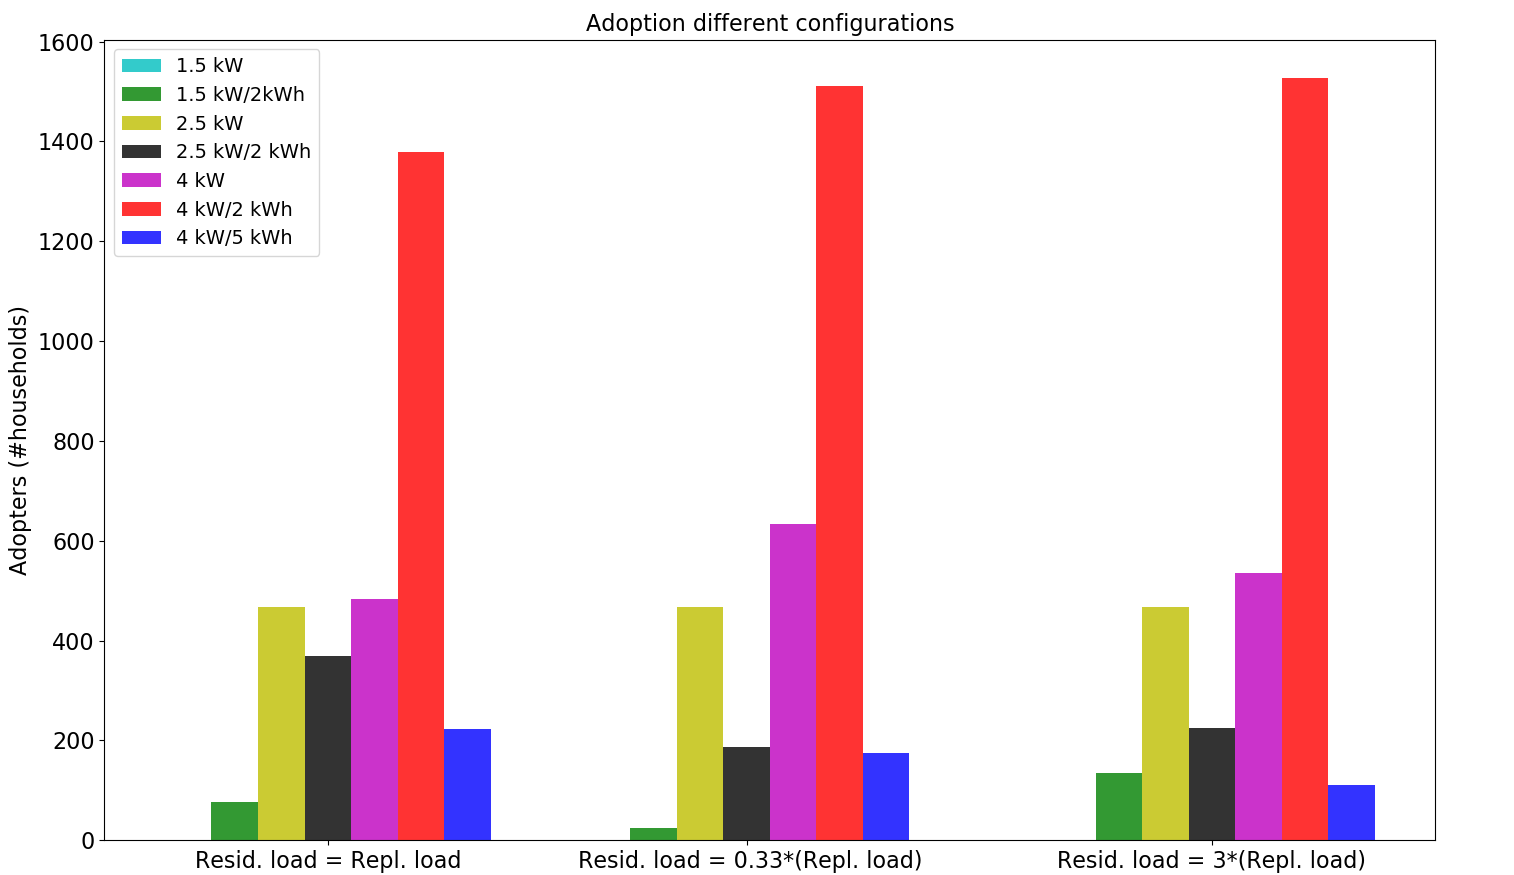
\includegraphics[width=10cm]{AppendixA/ConfigCapresid.PNG}
    \caption{Configurations for different residual loads}
    \label{fig:W}
\end{figure}
\noindent
\newline
\begin{figure}[h!]
    \centering
    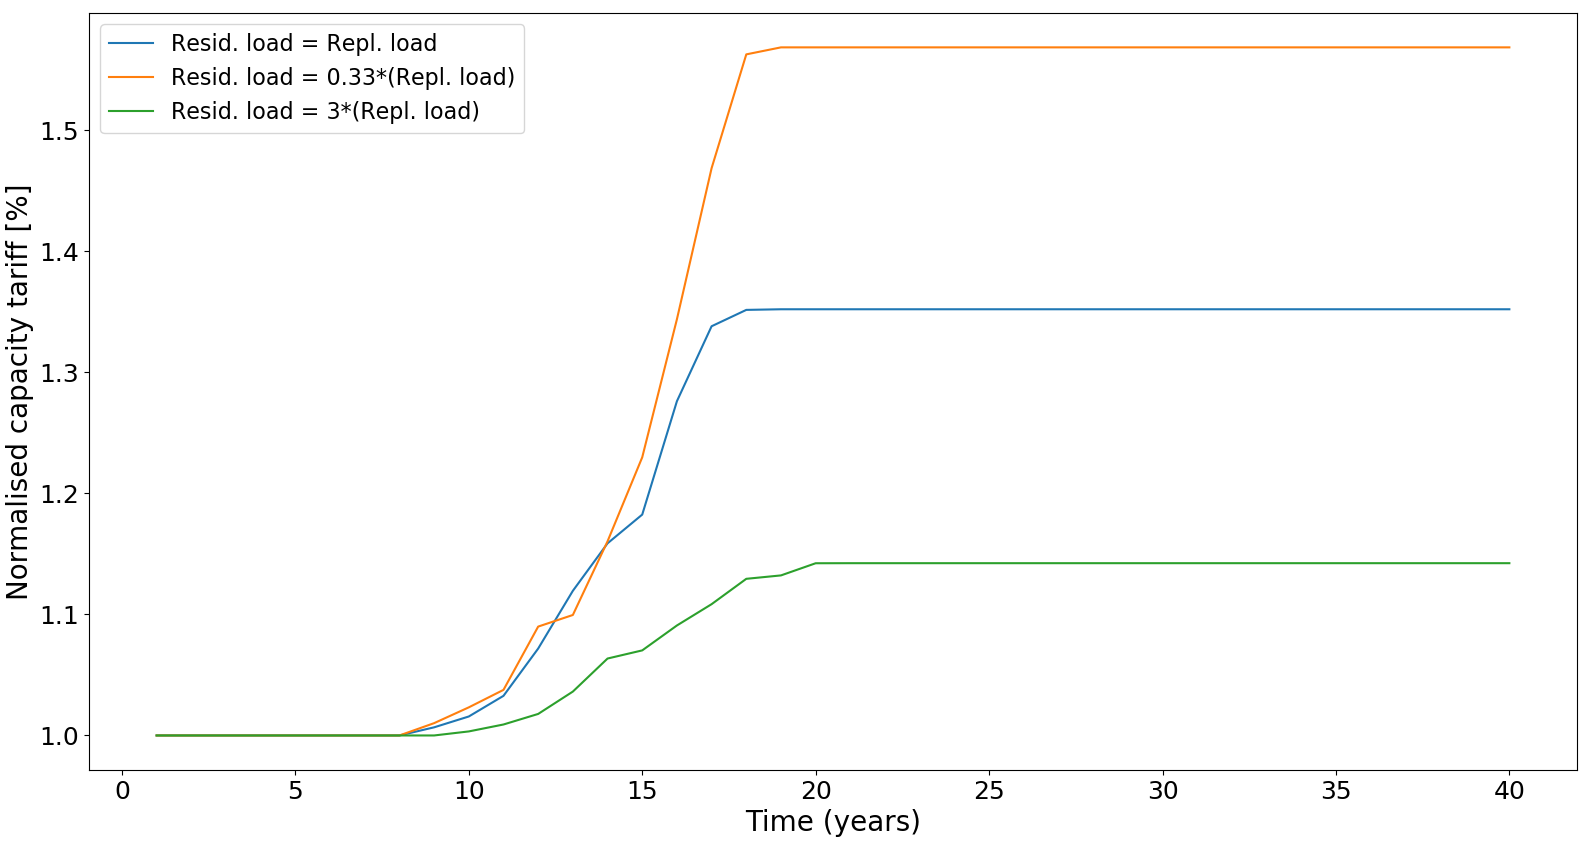
\includegraphics[width=10cm]{AppendixA/CapTarresid.PNG}
    \caption{Normalised distribution tariff for different residual loads}
    \label{fig:X}
\end{figure}
